\section{分类定理}
\label{ch12-sec77}

在本节中, 我们论述曲面分类定理的几何部分. 我们将证明通过成对黏合一个多边形区域的边所得到的空间同胚于 $S^{2}$、$n$-重环面 $T_{n}$ 或 $m$-重射影平面 $P_{m}$. 稍后, 我们还会说明为什么每一个紧致曲面都可以通过这种办法得到.

设 $w_{1},\ \cdots,\ w_{k}$ 为多边形区域 $P_{1},\ \cdots,\ P_{k}$ 的标记表. 如果在上述标记表中每一个标签恰好出现两次, 我们称这个标记表为\textbf{恰当}(proper)标记表. 注意以下重要事实:

\begin{remark}
一个恰当的标记表经过初等运算后, 得到的仍然是一个恰当的标记表.
\end{remark}

\begin{definition}[环型与射影型]
\label{definition:ch12-torus-projective-type}
设 $w$ 是某单一多边形区域的一个恰当的标记表. 我们称 $w$ 为\textbf{环型}(torus type)的标记表, 如果对于每一个标签而言 $+1$ 和 $-1$ 作为指数各出现一次. 否则, 我们称 $w$ 为\textbf{射影型}(projective type)的标记表.
\end{definition}

首先考虑一个射影型的标记表 $w$. 我们将证明 $w$ 等价于这样一个(具有相同长度的)标记表, 在这个标记表中每一个具有相同指数的同一个标签成对地出现在这个标记表的前部. 也就是说, $w$ 等价于一个具有以下形式的标记表
\[
(a_{1}a_{1})(a_{2}a_{2})\cdots(a_{k}a_{k})w_{1},
\]
其中 $w_{1}$ 或者是环型的或者是空的.

因为 $w$ 是射影型的, 那么标记表 $w$ 中至少有一个标签, 比如说标签 $a$, 使得在它出现的两个地方指数相同. 我们可设 $w$ 具有以下形式:
\[
w=y_{0}ay_{1}ay_{2},
\]
其中某一个 $y_{i}$ 可能为空. 为看起来方便, 我们在上述表达式中添加若干个括号, 将其表示为
\[
w=[y_{0}]a[y_{1}]a[y_{2}].
\]
我们有以下结论.

\begin{lemma}[射影型标签的配对]
\label{lemma:ch12-pair-projective}
设 $w$ 是一个以下形式的恰当的标记表:
\[
w=[y_{0}]a[y_{1}]a[y_{2}],
\]
其中某一个 $y_{i}$ 可能为空, 则它有一个等价形式
\[
w\sim aa[y_{0}y_{1}^{-1}y_{2}],
\]
其中 $y_{1}^{-1}$ 表示 $y_{1}$ 的形式逆.
\end{lemma}

\par
\begin{figure}[htbp]
\centering
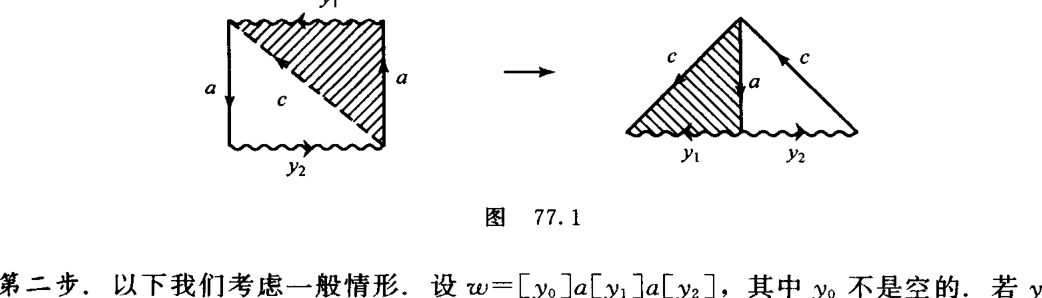
\includegraphics[width=0.6\textwidth]{image/fig-77-1.png}
\caption{$y_{0}$ 为空时的切割与黏合.}
\label{ch12-fig-77-1}
\end{figure}

\par
\begin{figure}[htbp]
\centering
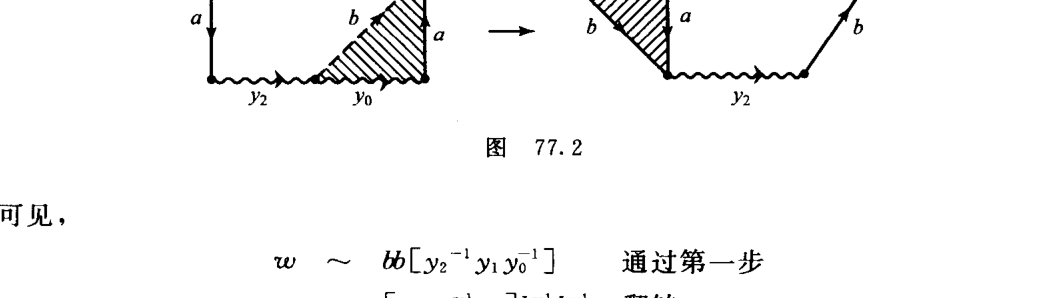
\includegraphics[width=0.7\textwidth]{image/fig-77-2.png}
\caption{一般情形的切割与黏合.}
\label{ch12-fig-77-2}
\end{figure}

\begin{proof}
\textbf{第一步.} 我们首先考虑 $y_{0}$ 为空的情形. 证明
\[
a[y_{1}]a[y_{2}]\sim aa[y_{1}^{-1}y_{2}].
\]
若 $y_{1}$ 是空的, 这是显然的. 若 $y_{2}$ 是空的, 可以经翻转、置换、换标签的方法得到等价性. 如果二者都非空, 可经切割、黏合、换标签得到等价性, 如\cref{ch12-fig-77-1} 所示. 请读者自己给出相应的初等运算.


\textbf{第二步.} 以下我们考虑一般情形. 设 $w=[y_{0}]a[y_{1}]a[y_{2}]$, 其中 $y_{0}$ 不是空的. 若 $y_{1}$ 和 $y_{2}$ 都是空的, 通过置换, 可见引理成立. 否则, 通过\cref{ch12-fig-77-2} 所示的切割和黏合得到
\[
w\sim b[y_{2}]b[y_{1}y_{0}^{-1}].
\]


由此可见,
\begin{align*}
w\quad&\sim\quad bb[y_{2}^{-1}y_{1}y_{0}^{-1}] &&\text{通过第一步}\\
&\sim\quad [y_{0}y_{1}^{-1}y_{2}]b^{-1}b^{-1} &&\text{翻转}\\
&\sim\quad aa[y_{0}y_{1}^{-1}y_{2}] &&\text{置换和换标签}.
\end{align*}
\end{proof}

\begin{corollary}[射影型标记表的标准形]
\label{corollary:ch12-projective-normal-form}
若 $w$ 是一个射影型标记表, 则 $w$ 等价于一个具有相同长度且形如
\[
(a_{1}a_{1})(a_{2}a_{2})\cdots(a_{k}a_{k})w_{1}
\]
的标记表, 其中 $k\geqslant 1$ 且 $w_{1}$ 为空或者是环型的.
\end{corollary}

\begin{proof}
标记表 $w$ 可以表示成以下形式:
\[
w=[y_{0}]a[y_{1}]a[y_{2}].
\]
前述引理蕴涵着 $w$ 等价于一个与其具有相同长度且形如 $w'=aaw_{1}$ 的标记表. 若 $w_{1}$ 是环型的, 则推论已经成立. 否则我们将 $w'$ 写成
\[
w'=aa[z_{0}]b[z_{1}]b[z_{2}]=[aaz_{0}]b[z_{1}]b[z_{2}]
\]
的形式. 再次应用前述引理, 可见 $w'$ 等价于 $w''$, 形如
\[
w''=bb[aaz_{0}z_{1}^{-1}z_{2}]=bbaaw_{2},
\]
其中 $w''$ 与 $w$ 具有相同长度. 若 $w_{2}$ 是环型的, 则结论已经成立. 否则, 继续进行类似的论证.
\end{proof}

按照上述推论, 若 $w$ 是某个多边形区域的一个恰当的标记表, 则 (1) $w$ 是环型的, 或 (2) $w$ 等价于形如 $(a_{1}a_{1})\cdots(a_{k}a_{k})w_{1}$ 的标记表, 其中 $w_{1}$ 是环型的, 或 (3) $w$ 等价于形如 $(a_{1}a_{1})\cdots(a_{k}a_{k})$ 的标记表. 对于情形 (3) 没有什么事情要做了, 因为这样的标记表表示若干个射影平面的连通和. 下面我们来讨论情形 (1) 和情形 (2).

为此, 我们注意若 $w$ 是情形 (1) 或情形 (2) 中所示的长度大于 $4$ 的标记表, 并且 $w$ 含有标签相同但指数相反的相邻的两项, 则可以经删除运算将其化为一个长度较短的如 (1), (2) 或 (3) 所示的标记表. 因此, 可将 $w$ 化为长度为 $4$ 的标记表或者相邻的标签皆互不相同的标记表.

我们将看到, 长度为 $4$ 的标记表是易于处理的. 因此我们假设 $w$ 不包含标签相同但指数相反的两项. 在这种情形下, 我们证明 $w$ 等价于一个具有相同长度的标记表 $w'$, 形如
\[
w'=aba^{-1}b^{-1}w''\qquad\text{对于情形 (1)}
\]
或
\[
w'=(a_{1}a_{1})\cdots(a_{k}a_{k})aba^{-1}b^{-1}w''\qquad\text{对于情形 (2)}
\]
其中 $w''$ 是环型的或者为空. 这是下列引理的主旨.

\begin{lemma}[环型部分的分离]
\label{lemma:ch12-separate-torus}
设 $w$ 是形如 $w=w_{0}w_{1}$ 的一个恰当的标记表, 其中 $w_{1}$ 为环型标记表, 并且没有相同的标签相邻. 则 $w$ 等价于形如 $w_{0}w_{2}$ 的标记表, 其中 $w_{2}$ 与 $w_{1}$ 具有相同的长度, 并且形如
\[
w_{2}=aba^{-1}b^{-1}w_{3},
\]
其中 $w_{3}$ 是环型的或者为空.
\end{lemma}

\par
\begin{figure}[htbp]
\centering
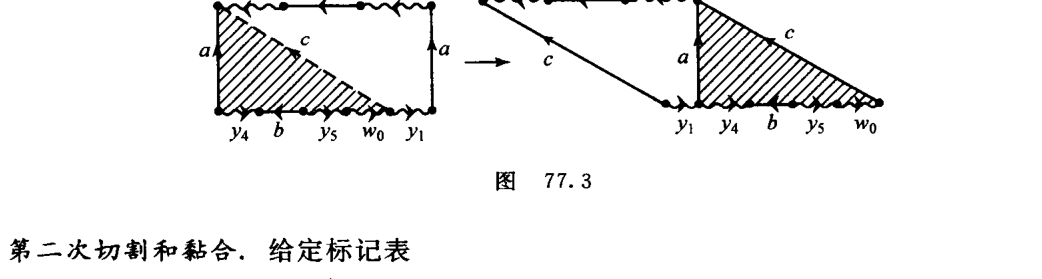
\includegraphics[width=0.8\textwidth]{image/fig-77-3.png}
\caption{第一次切割和黏合.}
\label{ch12-fig-77-3}
\end{figure}

\par
\begin{figure}[htbp]
\centering
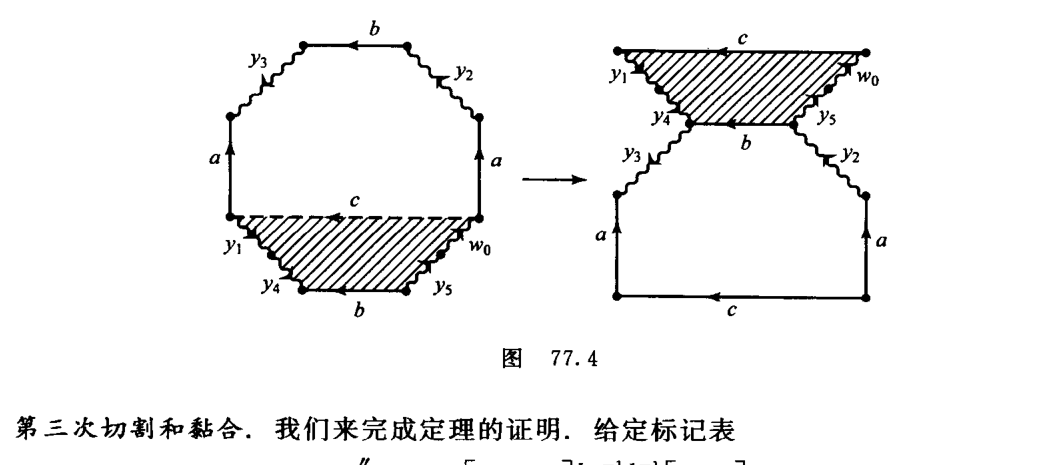
\includegraphics[width=0.8\textwidth]{image/fig-77-4.png}
\caption{第二次切割和黏合.}
\label{ch12-fig-77-4}
\end{figure}

\par
\begin{figure}[htbp]
\centering
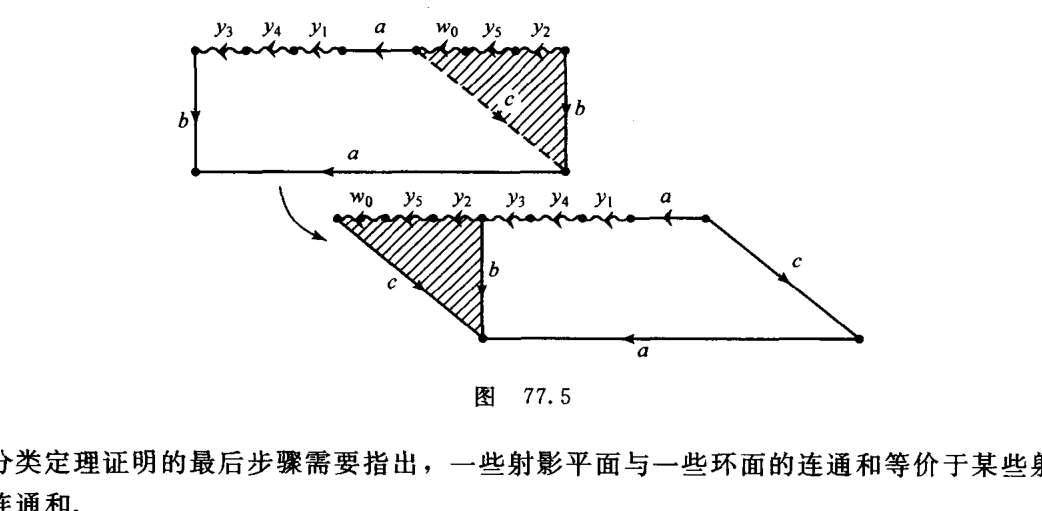
\includegraphics[width=0.85\textwidth]{image/fig-77-5.png}
\caption{第三次切割和黏合.}
\label{ch12-fig-77-5}
\end{figure}

\begin{proof}
这是本节最为精巧的一个证明, 它涉及三次切割和黏合. 我们先证明, 如果有必要的话, 需要适当地改变标签和指数, $w$ 可以写成
\[
w=w_{0}[y_{1}]a[y_{2}]b[y_{3}]a^{-1}[y_{4}]b^{-1}[y_{5}], \qquad (*)
\]
其中某一个 $y_{i}$ 可能是空的.

在 $w_{1}$ 所含的所有标签中, 设 $a$ 是一个出现两次的标签(它们的指数相反), 并且它们两次出现的位置最为接近. 根据假设这两次出现不是紧挨着的. 倘若有必要, 同时改变二者的指数, 可设 $a$ 在 $a^{-1}$ 的前面出现. 设 $b$ 是一个出现在 $a$ 与 $a^{-1}$ 之间的一个标签, 并设其指数为 $+1$. 此时 $b^{-1}$ 将出现在 $w_{1}$ 中, 但它不出现在 $a$ 与 $a^{-1}$ 之间, 这是由于 $a$ 和 $a^{-1}$ 出现的位置最为接近. 若 $b^{-1}$ 在 $a^{-1}$ 之后出现, 我们就得到结论. 若 $b^{-1}$ 在 $a$ 之前出现, 那么将每一个 $b$ 的指数改变符号, 然后再将标签 $a$ 与标签 $b$ 对调, 这样便得到了所需形式.

以下我们假定 $w$ 形如上式 $(*)$.

\textbf{第一次切割和黏合.} 我们证明 $w$ 等价于标记表
\[
w'=w_{0}a[y_{2}]b[y_{3}]a^{-1}[y_{1}y_{4}]b^{-1}[y_{5}].
\]
为此, 我们将 $w$ 改写为
\[
w=w_{0}[y_{1}]a[y_{2}by_{3}]a^{-1}[y_{4}b^{-1}y_{5}].
\]
使用\cref{ch12-fig-77-3} 所示的切割与黏合, 便有
\begin{align*}
w\quad&\sim\quad w_{0}c[y_{2}by_{3}]c^{-1}[y_{1}y_{4}b^{-1}y_{5}]\\
&\sim\quad w_{0}a[y_{2}]b[y_{3}]a^{-1}[y_{1}y_{4}]b^{-1}[y_{5}].
\end{align*}
这里用到了换标签的办法. 注意, 之所以可以在 $c$ 处切割, 是因为切割后的两个多边形都至少有三条边.


\textbf{第二次切割和黏合.} 给定标记表
\[
w'=w_{0}a[y_{2}]b[y_{3}]a^{-1}[y_{1}y_{4}]b^{-1}[y_{5}],
\]
我们证明 $w'$ 等价于标记表
\[
w''=w_{0}a[y_{1}y_{4}y_{3}]ba^{-1}b^{-1}[y_{2}y_{5}].
\]
若标记表 $y_{1}$, $y_{4}$, $y_{5}$ 及 $w_{0}$ 都是空的, 讨论很简单, 因为此时
\begin{align*}
w'\quad&=\quad a[y_{2}]b[y_{3}]a^{-1}b^{-1}\\
&\sim\quad b[y_{3}]a^{-1}b^{-1}a[y_{2}] &&\text{置换}\\
&\sim\quad a[y_{3}]ba^{-1}b^{-1}[y_{2}] &&\text{换标签}\\
&=\quad w''.
\end{align*}
否则, 用\cref{ch12-fig-77-4} 所示的运算得到
\begin{align*}
w'\quad&=\quad w_{0}a[y_{2}]b[y_{3}]a^{-1}[y_{1}y_{4}]b^{-1}[y_{5}]\\
&\sim\quad w_{0}c[y_{1}y_{4}y_{3}]a^{-1}c^{-1}a[y_{2}y_{5}]\\
&\sim\quad w_{0}a[y_{1}y_{4}y_{3}]ba^{-1}b^{-1}[y_{2}y_{5}],
\end{align*}
这里也用到了换标签的办法.


\textbf{第三次切割和黏合.} 我们来完成定理的证明. 给定标记表
\[
w''=w_{0}a[y_{1}y_{4}y_{3}]ba^{-1}b^{-1}[y_{2}y_{5}],
\]
我们证明 $w''$ 等价于标记表
\[
w'''=w_{0}aba^{-1}b^{-1}[y_{1}y_{4}y_{3}y_{2}y_{5}].
\]
若标记表 $w_{0}$, $y_{5}$, $y_{2}$ 都是空的, 证明很容易, 因为在这种情形下
\begin{align*}
w''\quad&=\quad a[y_{1}y_{4}y_{3}]ba^{-1}b^{-1}\\
&\sim\quad ba^{-1}b^{-1}a[y_{1}y_{4}y_{3}] &&\text{置换}\\
&\sim\quad aba^{-1}b^{-1}[y_{1}y_{4}y_{3}] &&\text{换标签}\\
&=\quad w'''.
\end{align*}
否则, 我们按照\cref{ch12-fig-77-5} 所示的运算得到
\begin{align*}
w''\quad&=\quad w_{0}a[y_{1}y_{4}y_{3}]ba^{-1}b^{-1}[y_{2}y_{5}]\\
&\sim\quad w_{0}ca^{-1}c^{-1}a[y_{1}y_{4}y_{3}y_{2}y_{5}]\\
&\sim\quad w_{0}aba^{-1}b^{-1}[y_{1}y_{4}y_{3}y_{2}y_{5}],
\end{align*}
式中再一次用到了换标签的办法. 定理证毕.

\end{proof}

分类定理证明的最后步骤需要指出, 一些射影平面与一些环面的连通和等价于某些射影平面的连通和.

\begin{lemma}[环面与射影平面的交换]
\label{lemma:ch12-torus-projective-swap}
设 $w$ 是一个恰当的标记表, 形如
\[
w=w_{0}(cc)(aba^{-1}b^{-1})w_{1},
\]
则 $w$ 等价于标记表
\[
w'=w_{0}(aabbcc)w_{1}.
\]
\end{lemma}

\begin{proof}
在 \cref{lemma:ch12-pair-projective} 中我们曾经得到: 对恰当的标记表, 我们有
\[
[y_{0}]a[y_{1}]a[y_{2}]\sim aa[y_{0}y_{1}^{-1}y_{2}]. \qquad (*)
\]
本引理的证明如下:
\begin{align*}
w\quad&\sim\quad (cc)(aba^{-1}b^{-1})w_{1}w_{0} &&\text{置换}\\
&=\quad cc[ab][ba]^{-1}[w_{1}w_{0}]\\
&\sim\quad [ab]c[ba]c[w_{1}w_{0}] &&\text{根据 $(*)$, 从后向前看}\\
&=\quad [a]b[c]b[acw_{1}w_{0}]\\
&\sim\quad bb[ac^{-1}acw_{1}w_{0}] &&\text{根据 $(*)$}\\
&=\quad [bb]a[c]^{-1}a[cw_{1}w_{0}]\\
&\sim\quad aa[bbccw_{1}w_{0}] &&\text{根据 $(*)$}\\
&\sim\quad w_{0}aabbccw_{1} &&\text{置换}.
\end{align*}
\end{proof}

\begin{theorem}[分类定理]
\label{theorem:ch12-classification}
设 $X$ 是通过成对地黏合平面多边形区域的边所获得的商空间, 则 $X$ 同胚于 $S^{2}$、$n$-重环面 $T_{n}$ 或 $m$-重射影平面 $P_{m}$.
\end{theorem}

\begin{proof}
设 $w$ 是多边形区域 $P$ 的用来得到空间 $X$ 的那个标记表. 这时 $w$ 是一个长度不小于 $4$ 的恰当的标记表. 我们证明 $w$ 等价于下列标记表之一:
\begin{enumerate}[(1)]
\item $aa^{-1}bb^{-1}$.
\item $abab$.
\item $(a_{1}a_{1})(a_{2}a_{2})\cdots(a_{m}a_{m})$, 其中 $m\geqslant 2$.
\item $(a_{1}b_{1}a_{1}^{-1}b_{1}^{-1})(a_{2}b_{2}a_{2}^{-1}b_{2}^{-1})\cdots(a_{n}b_{n}a_{n}^{-1}b_{n}^{-1})$, 其中 $n\geqslant 1$.
\end{enumerate}
第一个标记表给出空间 $S^{2}$, 第二个标记表给出空间 $P^{2}$, 第 74 节的\cref{example:ch12-triangle-sphere} 和\cref{example:ch12-projective-plane} 中曾经提到过. 第三个标记表和第四个标记表分别给出空间 $P_{m}$ 和 $T_{n}$.

\textbf{第一步.} 设 $w$ 为环型标记表. 我们证明 $w$ 等价于标记表 (1) 或 (4) 型标记表.

若 $w$ 的长度为 $4$, 则它可以写成下列两种形式之一:
\[
aa^{-1}bb^{-1}\qquad\text{或者}\qquad aba^{-1}b^{-1}.
\]
前一种为 (1) 型, 后一种属于 (4) 型.

以下我们对 $w$ 的长度进行归纳. 假设 $w$ 的长度大于 $4$. 若 $w$ 等价于一个较短的环型标记表, 那么根据归纳假设便得到了所需结论. 否则, $w$ 是不包含在相邻的位置上出现相同标签的标记表. 应用 \cref{lemma:ch12-separate-torus} (对 $w_{0}$ 为空的情形) 可见, $w$ 等价于一个与其具有相同长度的标记表, 形如
\[
aba^{-1}b^{-1}w_{3},
\]
其中 $w_{3}$ 是环型的. 由于 $w$ 的长度大于 $4$, 从而 $w_{3}$ 非空. 并且 $w_{3}$ 中也不包含在相邻的位置上出现相同标签的标记表, 因为 $w$ 不等价于较短的环型标记表. 对于 $w_{0}=aba^{-1}b^{-1}$ 再次应用 \cref{lemma:ch12-separate-torus}, 我们得到 $w$ 等价于一个标记表, 形如
\[
(aba^{-1}b^{-1})(cdc^{-1}d^{-1})w_{4},
\]
其中 $w_{4}$ 为空或者是环型的. 若 $w_{4}$ 为空, 则我们已经完成了证明. 否则再次应用 \cref{lemma:ch12-separate-torus} 继续类似的讨论.

\textbf{第二步.} 假设 $w$ 为射影型的恰当的标记表. 我们证明 $w$ 等价于标记表 (2) 或者等价于 (3) 型标记表.

若 $w$ 的长度为 $4$, 则 \cref{corollary:ch12-projective-normal-form} 蕴涵着 $w$ 等价于标记表 $aabb$ 或 $aab^{-1}b$. 前者是属于类型 (3) 的一个标记表. 后者可以表示成形如 $aay_{1}^{-1}y_{2}$, 其中 $y_{1}=y_{2}=b$, 这时 \cref{lemma:ch12-pair-projective} 蕴涵着它等价于标记表 $ay_{1}ay_{2}=abab$, 即标记表 (2).

对 $w$ 的长度进行归纳. 假设 $w$ 的长度大于 $4$. \cref{corollary:ch12-projective-normal-form} 告诉我们 $w$ 等价于形如
\[
w'=(a_{1}a_{1})\cdots(a_{k}a_{k})w_{1}
\]
的标记表, 其中 $k\geqslant 1$ 并且 $w_{1}$ 是环型的或者为空. 若 $w_{1}$ 为空, 我们就完成了证明. 若 $w$ 中含有紧挨着的两个相同的标签, 则 $w'$ 等价于一个具有较短长度的射影型标记表, 因而可以运用归纳假设证得结论. 否则, \cref{lemma:ch12-separate-torus} 蕴涵着 $w'$ 等价于以下形式的标记表:
\[
w''=(a_{1}a_{1})\cdots(a_{k}a_{k})aba^{-1}b^{-1}w_{2},
\]
其中 $w_{2}$ 为空或者是环型的. 这时我们应用 \cref{lemma:ch12-torus-projective-swap} 得到 $w''$ 与以下标记表等价:
\[
(a_{1}a_{1})\cdots(a_{k}a_{k})aabbw_{2}.
\]
继续类似的论证, 最终我们将会得到属于类型 (3) 的一个标记表.
\end{proof}

\begin{exercise}
\label{exercise:ch12-sec77-01}
设 $X$ 是通过成对地黏合某多边形区域的边所得到的空间.
\begin{enumerate}[(a)]
\item 证明 $X$ 恰好同胚于下列空间之一: $S^{2}$, $P^{2}$, $K$, $T_{n}$, $T_{n}\#P^{2}$, $T_{n}\#K$, 其中 $K$ 是 Klein 瓶, $n\geqslant 1$.
\item 证明 $X$ 恰好同胚于以下空间之一: $S^{2}$, $T_{n}$, $P^{2}$, $K_{m}$, $P^{2}\#K_{m}$, 其中 $K_{m}$ 是 $K$ 的 $m$-重连通和, $m\geqslant 1$.
\end{enumerate}
\end{exercise}

\begin{exercise}
\label{exercise:ch12-sec77-02}
\begin{enumerate}[(a)]
\item 写出由\cref{ch12-fig-77-1} 和\cref{ch12-fig-77-2} 所示变换过程中用到的初等运算序列.
\item 写出由\cref{ch12-fig-77-3}、\cref{ch12-fig-77-4} 和\cref{ch12-fig-77-5} 所示变换过程中用到的初等运算序列.
\end{enumerate}
\end{exercise}

\begin{exercise}
\label{exercise:ch12-sec77-03}
分类定理的证明提供了一种算法, 将给定多边形区域的一个恰当的标记表化为定理中的 $4$ 种标准形式之一. 其相应的等价关系如下:
\begin{enumerate}[(i)]
\item $[y_{0}]a[y_{1}]a[y_{2}]\sim aa[y_{0}y_{1}^{-1}y_{2}]$.
\item $[y_{0}]aa^{-1}[y_{1}]\sim [y_{0}y_{1}]$, 如果 $y_{0}y_{1}$ 的长度不小于 $4$.
\item $w_{0}[y_{1}]a[y_{2}]b[y_{3}]a^{-1}[y_{4}]b^{-1}[y_{5}]\sim w_{0}aba^{-1}b^{-1}[y_{1}y_{4}y_{3}y_{2}y_{5}]$.
\item $w_{0}(cc)(aba^{-1}b^{-1})w_{1}\sim w_{0}aabbccw_{1}$.
\end{enumerate}
使用以上算法, 将下列标记表化为标准形式.
\begin{enumerate}[(a)]
\item $abacb^{-1}c^{-1}$.
\item $abca^{-1}cb$.
\item $abbca^{-1}ddc^{-1}$.
\item $abcda^{-1}b^{-1}c^{-1}d^{-1}$.
\item $abcda^{-1}c^{-1}b^{-1}d^{-1}$.
\item $aabcc^{-1}b^{-1}d^{-1}$.
\item $abcdabdc$.
\item $abcdabcd$.
\end{enumerate}
\end{exercise}

\begin{exercise}
\label{exercise:ch12-sec77-04}
设 $w$ 是某 $10$-边形区域的一个恰当的标记表. 若 $w$ 是射影型的, 那么它能表示成 \cref{theorem:ch12-classification} 中的哪些空间? 当 $w$ 为环型时, 结论又如何?
\end{exercise}
